% ---------------------------------------------------------------------------
\newpage
\hypertarget{appendix-using-sage}{}
\section{Using Sage with this Script}
\label{s:appendix-using-sage}
\index{Sage}
\index{Sage!Code examples}

This script includes numerous code samples using Sage. Sage is an open
source computer algebra system (CAS) that supports teaching, study and
research in mathematics.  It combines many high-quality open
source packages\footnote{%
To get an impression, how big Sage is: After downloading the source of Sage 4.1,
it took around 5 h on a average Linux PC to compile the whole system including
all libraries, and it occupied 1.8 GB disk space then.
}
and provides access to their functionalities via a
common interface, namely, a Python\footnote{%
There is also an easy interface to the C language, called Cython, which can be used
to speed up own functions in Sage very much.\\
See \url{http://openwetware.org/wiki/Open_writing_projects/Sage_and_cython_a_brief_introduction}.
} based programming language.

\noindent Sage can be used as a powerful desktop calculator, as a tool to help
(undergraduate) students study mathematics, or as a programming
environment for prototyping algorithms and research in algorithmic
aspects of mathematics.

\noindent You can get a quick impression of Sage e.g. with David Joyner's
``Invitation to Sage''\footnote{%
\url{http://sage.math.washington.edu/home/wdj/teaching/calc1-sage/an-invitation-to-sage.pdf}\\
(last update 2009).}.
  
\noindent The official Sage online documentation\footnote{%
  The according official PDF documents can be downloaded at\\
  \url{http://www.sagemath.org/help.html}
} is available at: \url{http://www.sagemath.org/doc}.


%% \centering statt \begin{center} ... \end{center}, da dies zus�tzlich vertical space erzeugt.
\noindent In the meantime there are lots of PDF or HTML documents about using Sage,
so we name only a few of them: A good starting point is the ``Library''
from the Sage main page, the ``Documentation Project'' and the teaching
material\footnote{%
- ``Library'': {\centering \url{http://www.sagemath.org/library/index.html}},\\
- ``Documentation Project'': {\centering \url{http://wiki.sagemath.org/DocumentationProject}},\\
- ``Teaching'': {\centering \url{http://wiki.sagemath.org/Teaching_with_SAGE}}.
}.

\noindent With respect to studying cryptography, Sage modules can be used
to complement a first course in cryptography\footnote{%
- Module sources in the directory \url{SAGE_ROOT/devel/sage-main/sage/crypto}.\\
- Overview, what crypto currently is in Sage:\\
~ ~ \url{http://www.sagemath.org/doc/reference/sage/crypto/}\\
- Discussions about the teaching related aspect of development crypto in Sage:\\
~ ~ \url{http://groups.google.com/group/sage-devel/browse_thread/thread/c5572c4d8d42d081}
}.

\noindent Especially David Kohel's notes at\\
{\centering \url{http://www.sagemath.org/library/crypto.pdf} }
or the same eventually newer at\\
{\centering \url{http://sage.math.washington.edu/home/wdj/teaching/kohel-crypto.pdf} }\\
can be used to teach such a course that incorporates Sage.


% ---------------------------------------------------------------------------
\section*{Sage user interfaces}
Sage is available free of charge and can be downloaded from the
following website:
\begin{center}
  \url{http://www.sagemath.org} \\
\end{center}
The default interface to Sage is command line based, as shown in
Figure~\ref{fig:sage_cmd_interfaces}. However, there is a
graphical user interface to the software as well in the form of the
Sage notebook (see Figure~\ref{fig:sage_gui_interfaces}). We can even
use Sage online at different servers, e.g.
\begin{center}
\url{http://www.sagenb.org}
\url{http://sage.mathematik.uni-siegen.de:8000}
\end{center}
without having to install Sage locally.

Sage runs under many Linux distributions, Mac OS X, and Windows.
For the Windows platform, a complete distribution of Sage currently
only runs as a VMware image. However, a full native port of Sage
to Windows is currently in progress.

\begin{figure}[!htpb]
\centering
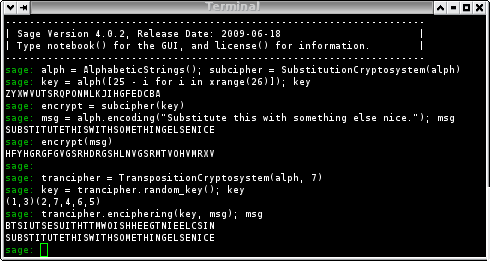
\includegraphics[scale=0.6]{figures/sage-cmd}
\caption{Sage command line interface}
\label{fig:sage_cmd_interfaces}
\end{figure}

\begin{figure}[!htpb]
\centering
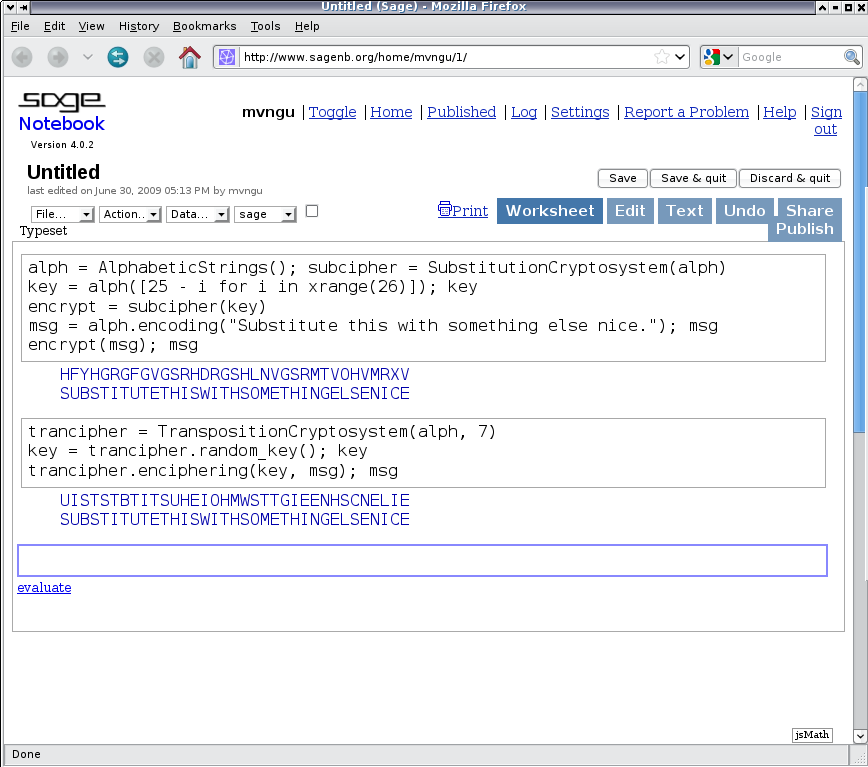
\includegraphics[scale=0.4]{figures/sage-gui}
\caption[Sage notebook interface]{Sage notebook interface\footnotemark}
\label{fig:sage_gui_interfaces}
\end{figure}

\footnotetext{%
To start the Sage gui: Enter notebook() at the Sage prompt, and then your favorite
browser (Iceweasel, Firefox, IE, ...) is started e.g. with the URL \url{http://localhost:8000}.
}



% ---------------------------------------------------------------------------
\newpage
\section*{Getting help with using Sage}

Upon loading Sage from the command line, we are presented with
something similar to the following:
%
\begin{Verbatim}%
[fontsize=\footnotesize,fontshape=tt]
mnemonic:~$ sage
----------------------------------------------------------------------
| Sage Version 4.1, Release Date: 2009-07-09                         |
| Type notebook() for the GUI, and license() for information.        |
----------------------------------------------------------------------

sage: help
Type help() for interactive help, or help(object) for help about object.
sage:
sage:
sage: help()

Welcome to Python 2.6!  This is the online help utility.

If this is your first time using Python, you should definitely check out
the tutorial on the Internet at http://docs.python.org/tutorial/.

Enter the name of any module, keyword, or topic to get help on writing
Python programs and using Python modules.  To quit this help utility and
return to the interpreter, just type "quit".

To get a list of available modules, keywords, or topics, type "modules",
"keywords", or "topics".  Each module also comes with a one-line summary
of what it does; to list the modules whose summaries contain a given word
such as "spam", type "modules spam".
\end{Verbatim}
%
Plenty of help is provided in the form of the official Sage
documentation that is distributed with every release of Sage~(see
Figure~\ref{fig:sage_standard_doc}).
%
\begin{figure}[!htpb]
\centering
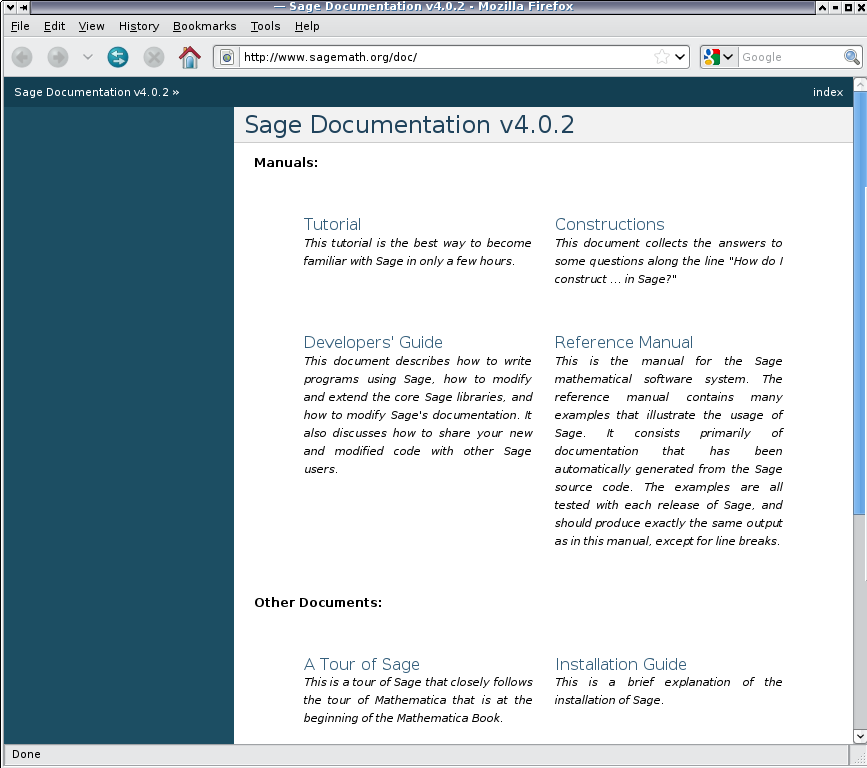
\includegraphics[scale=0.4]{figures/sage-online-doc}
\caption{The Sage standard documentation}
\label{fig:sage_standard_doc}
\end{figure}
%
The official Sage standard documentation includes the following documents:

\begin{itemize}
\item Tutorial --- This tutorial is designed to help Sage beginners
  become familiar with Sage. It covers many features that beginners
  should be familiar with, and takes one to three hours to go through.

\item Constructions --- This document is in the style of a Sage
  ``cookbook''. It is a collection of answers to questions about
  constructing various objects in Sage.

\item Developers' Guide --- This guide is for developers who want to
  contribute to the development of Sage. Among other issues, it covers
  coding style and conventions, modifying the core Sage libraries,
  modifying the Sage standard documentation, and code review and
  distribution.

\item Reference Manual --- This manual provides complete documentation
  on the major features of Sage. The description of a class is
  accompanied by numerous code samples. All code samples in the
  reference manual are tested before each Sage release.

\item Installation Guide --- This guide explains how to install Sage
  under various platforms.

\item A Tour of Sage --- This is a tour of Sage that showcases various
  features of Sage that are useful for beginners.

\item Numerical Sage --- This document introduces tools available
  under Sage that are useful for numerical computation.

\item Three Lectures about Explicit Methods in Number Theory Using
  Sage --- This document is about using Sage to perform computations
  in advanced number theory.
\end{itemize}

\noindent From within a Sage session, we can obtain a list of commands matching
some pattern.  To do so, we type the first few characters and then
press the ``Tab'' key:
%
\begin{Verbatim}%
[fontsize=\footnotesize,fontshape=tt]
sage: Su[TAB]
Subsets                   Subwords                  SuzukiGroup
SubstitutionCryptosystem  SupersingularModule
\end{Verbatim}
%
If we know the exact name of a command, we can use the \texttt{help}
function to obtain further information on that command, or append the
question mark ``?'' to the command name.  For example,
the command \texttt{help(SubstitutionCryptosystem)} provides
documentation on the built-in class
\texttt{SubstitutionCryptosystem}. We can get documentation on
this class with the question mark as follows:
%
\begin{Verbatim}%
[fontsize=\footnotesize,fontshape=tt]
sage: SubstitutionCryptosystem?
Type:type
Base Class:<type 'type'>
String Form:<class 'sage.crypto.classical.SubstitutionCryptosystem'>
Namespace:Interactive
File:/home/mvngu/usr/bin/sage-3.4.1/local/lib/python2.5/site-packages/sage/crypto/classical.py
Docstring:

        Create a substitution cryptosystem.

        INPUT:

        - ``S`` - a string monoid over some alphabet

        OUTPUT:

        - A substitution cryptosystem over the alphabet ``S``.

        EXAMPLES::

            sage: M = AlphabeticStrings()
            sage: E = SubstitutionCryptosystem(M)
            sage: E
            Substitution cryptosystem on Free alphabetic string monoid
            on A-Z
            sage: K = M([ 25-i for i in range(26) ])
            sage: K
            ZYXWVUTSRQPONMLKJIHGFEDCBA
            sage: e = E(K)
            sage: m = M(``THECATINTHEHAT'')
            sage: e(m)
            GSVXZGRMGSVSZG

        TESTS::

            sage: M = AlphabeticStrings()
            sage: E = SubstitutionCryptosystem(M)
            sage: E == loads(dumps(E))
            True
\end{Verbatim}
%
\vspace{30pt}
For further assistance on specific problems, we can also
search the archive of the \texttt{sage-support} mailing list at
%
\begin{center}
  \url{http://groups.google.com/group/sage-support}
\end{center}




% ---------------------------------------------------------------------------
\newpage
\section*{Some examples using the built-in mathematical functions in Sage}

Here are a few little examples\footnote{%
The examples are from the blog of Prof. Alasdair McAndrew, Victoria University,\\
\url{http://amca01.wordpress.com/2008/12/19/sage-an-open-source-mathematics-software-system}}
(all in console mode, for ease) to see what you can do with Sage:

\begin{sagecode}
\begin{Verbatim}%
[fontsize=\footnotesize,fontshape=tt]
# * Calculus:
    sage: x=var('x')
    sage: p=diff(exp(x^2),x,10)*exp(-x^2)
    sage: p.simplify_exp()
     1024 x^10 + 23040 x^8 + 161280 x^6 + 403200 x^4 + 302400 x^2 + 30240

# * Linear Algebra:
    sage: M=matrix([[1,2,3],[4,5,6],[7,8,10]])
    sage: c=random_matrix(ZZ,3,1);c
     [ 7 ]
     [-2 ]
     [-2 ]
    sage: b=M*c
    sage: M^-1*b
     [ 7 ]
     [-2 ]
     [-2 ]

# * Number theory:
    sage: p=next_prime(randint(2^49,2^50));p
      1022095718672689
    sage: r=primitive_root(p);r
      7
    sage: pl=log(mod(10^15,p),r);pl
      1004868498084144
    sage: mod(r,p)^pl
      1000000000000000

# * Finite Fields (\url{http://en.wikipedia.org/wiki/Finite_field}):
    sage: F.<x>=GF(2)[]
    sage: G.<a>=GF(2^4,name='a',modulus=x^4+x+1)
    sage: a^2/(a^2+1)
      a^3 + a
    sage: a^100
      a^2 + a + 1
    sage: log(a^2,a^3+1)
      13
    sage: (a^3+1)^13
      a^2
\end{Verbatim}
\caption{Some small general samples in Sage from different areas in mathematics}
\end{sagecode}






% ---------------------------------------------------------------------------
\newpage
\section*{Writing code samples with Sage}

At the beginning using a CAS (computer algebra system) you type in the single commands
on the command line as in the above example\footnote{%
  The standard way for presenting Sage code starts the lines with ``sage:'' and ``...''.
  \begin{Verbatim}%
  [fontsize=\footnotesize,fontshape=tt]
  sage: m = 11
  sage: for a in xrange(1, m):
  ....:     print [power_mod(a, i, m) for i in xrange(1, m)]
  ....:
  \end{Verbatim}

  \noindent This script usually uses the above convention for presenting Sage code,
  if the code doesn't come from a Sage script. When people copy and paste the Sage code
  from the this script, in order to enter it a the commandline, 
  they should leave out "sage:" and "..."from the script (nevertheless
  in most cases the command prompt can deal with this prefixes correctly).}.

But if you develop your own functions, modify them and call them, then it is much easier
to do the development in your own editor, save it to a script file and execute the functions
non-interactively on the commandline manually.
Both ways to develop code is done in the examples in
chapter \ref{PaP_Sage_samples} (``\nameref{PaP_Sage_samples}'') and in
chapter \ref{NumberTheory_Appendix_E} (``\nameref{NumberTheory_Appendix_E}'').

\noindent To program and test Sage code using an editor there are two useful commands:
load() and attach()\footnote{%
See Sage tutorial about Programming, chapter ``Loading and Attaching SAGE files'',\\
\url{http://www.sagemath.org/doc/tutorial/programming.html\#loading-and-attaching-sage-files}.}.\\
Suppose you have a function definition like this:
\begin{Verbatim}%
   [fontsize=\footnotesize,fontshape=tt]
   def function(var1):
       r"""
       DocText.
       """
       ...
       return (L)
\end{Verbatim}
\noindent which has been saved to the file \texttt{primroots.sage}.

\noindent To load this function into Sage (and do a syntax check at once), use load() as follows:

\texttt{sage: load primroots.sage}

\noindent and you can then proceed to use on the command line anything that is
defined in that Sage script\footnote{%
Notes:
Don't use white spaces in your file name.\\
Its recommended that your Sage script has the file extension
``.sage'', instead of ``.py''. With a Sage script whose file name ends in
``.sage'', when you load it into Sage then the default Sage environment
is also loaded to make sure that it works as if you have defined your
function from the Sage command line. This also applies if you run the
script from a bash shell using ~~ \texttt{\$ sage primroots.sage}.

If you run your script as above, then Sage first parses your script,
writes it to another file called ``primroots.py'' (note the ``.py''
extension), adds all necessary variables to "primroots.py" as well as
writing any import statements to that file. That way, your Sage script
is executed as if you had typed the definitions in your script to the
Sage command line. A diffeence may be, that output needs a print statement.}.

Normally we also want to edit an own Sage script and reload the
content of the changed script into Sage again. In that case, you can
use the command attach(). Going back to our example of the above
function definition, say now you attach it to a Sage session as
follows (you also can apply atach() directly after laoding the script,
even before having changed the script):

\texttt{sage: attach primroots.sage}

Now edit the Sage script in a text editor, but don't exit Sage.
After you saved it within your text editor, the changed function
definition is reloaded into the running Sage session after the
next typing of Enter (and a syntax check is done at once). This reloading is
done automatically for you, provided that all changes to your script
have been saved. You can think of the command attach() as a way of
telling Sage to watch for all changes to a file, and reloading the
file again once Sage notices that there have been changes. With this
command, you don't have to copy and paste between your text editor and
the Sage command line interface.

Here is a picture of Sage code in the editor GVIM with activated code highlighting
~(see Figure~\ref{fig:sage-highlighted-code-in-editor}).
%
\begin{figure}[!htpb]
\centering
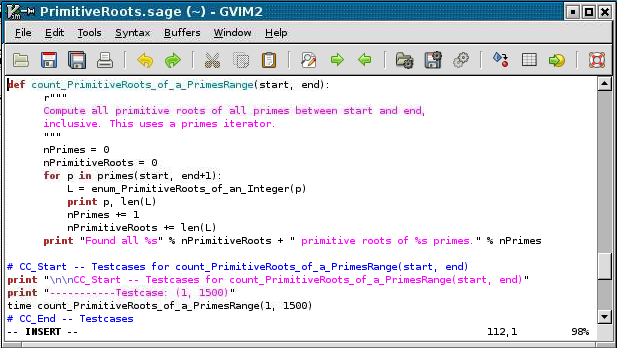
\includegraphics[scale=0.7]{figures/sage-highlighted-code-in-editor}
\caption{Sage sample shown in an editor with code highlighting}
\label{fig:sage-highlighted-code-in-editor}
\end{figure}


\vspace{30pt}
To get the version of your Sage environment:
\\texttt{version()}


To move quickly to the Sage code examples in this script, either look in the
index at \verb#Sage -> Code examples#, or have a look at the appendix
``\nameref{sc:List-of-Sage-Code-Examples}''.


